% Kinect Lite: project report.
% Build (from this folder):  pdflatex report.tex  (run twice for references), then copy report.pdf to ../results.pdf
% Every number in this file comes from ../src/results/icl_compare.txt, ../src/results/tum_compare.txt
% and ../experiments/hole_filling/results/fills.txt.
\documentclass[11pt,a4paper]{article}

\usepackage[margin=2.3cm]{geometry}
\usepackage[T1]{fontenc}
\usepackage{lmodern}
\usepackage{microtype}
\usepackage{amsmath}
\usepackage{graphicx}
\usepackage{booktabs}
\usepackage{array}
\newcolumntype{L}[1]{>{\raggedright\arraybackslash}p{#1}}

\usepackage{multirow}
\usepackage{xcolor}
\usepackage{tikz}
\usetikzlibrary{positioning,arrows.meta,fit,backgrounds}
\usepackage{caption}
\captionsetup{font=small,labelfont=bf,margin=0.5cm}
\usepackage{enumitem}
\setlist{itemsep=2pt,topsep=4pt}
\usepackage{tcolorbox}
\usepackage[hidelinks]{hyperref}

\definecolor{ours}{HTML}{E07B00}
\definecolor{paper}{HTML}{C0392B}
\definecolor{boxbg}{HTML}{F3F6FA}
\definecolor{boxframe}{HTML}{4A6A8A}
\newtcolorbox{keybox}[1][]{colback=boxbg,colframe=boxframe,boxrule=0.6pt,arc=2pt,
  left=6pt,right=6pt,top=4pt,bottom=4pt,fonttitle=\bfseries\small,#1}

\newcommand{\best}[1]{\textbf{#1}}
\usepackage{xspace}
\newcommand{\cm}{\,cm\xspace}
\newcommand{\mm}{\,mm\xspace}

\title{\textbf{Kinect Lite: Cleaning Kinect-Style Depth Images\\for Better Camera Tracking}\\[4pt]
\large A simple median filter vs.\ the spatial-temporal pipeline of Fu et al.\ (2012)}
\author{Mini Project Report}
\date{November 2026}

\begin{document}
\maketitle

% ---------------------------------------------------------------------------
\begin{abstract}
\noindent
Depth cameras such as the Kinect give a distance for every pixel, but the images contain
\emph{spikes} (pixels with a badly wrong distance) and \emph{holes} (pixels with no distance).
We compare two ways of cleaning the depth image: our own per-frame \textbf{9$\times$9 median filter}, and
the spatial-temporal denoising pipeline of \textbf{Fu et al.\ (2012)}. Instead of stopping at
``how close is the cleaned depth to the truth'', we also feed each cleaned sequence into two camera trackers,
one that uses depth only and one that uses colour and depth, and measure how far the estimated camera path drifts
from the true path. Tests use a synthetic dataset with true depth (ICL-NUIM) and a real-sensor dataset (TUM RGB-D).

\smallskip\noindent
\textbf{Findings.} (1) The median halves the depth error on ICL (18.8 vs.\ 39.2\mm; the paper: 37.7\mm).
(2) Which cleaner gives better tracking depends on the tracker: the paper's pipeline gives 4--16$\times$ less
drift with the depth-only tracker, and the median is best with the colour-plus-depth tracker (0.98\cm vs.\ 26.0\cm on ICL).
(3) Of eight ways to fill the remaining holes, none improves the colour-plus-depth tracker.
(4) The median runs in under a minute for 450 frames; the paper's pipeline takes about 26 minutes.
\end{abstract}

% ---------------------------------------------------------------------------
\section{Introduction}

A camera that moves through a room can work out its own path by lining up each new depth image with the previous one.
This is \emph{camera tracking} (also called visual odometry), and it is the first step of 3D scanning and
SLAM. Errors in the depth image lead to small errors in each step, and these add up to \emph{drift}.

Kinect-style sensors produce two kinds of depth error:
\begin{itemize}
  \item \textbf{Spikes:} single pixels or small clusters whose depth is wrong by centimetres to metres,
        mostly at object edges and on far or shiny surfaces.
  \item \textbf{Holes:} pixels where the sensor returns no depth at all, e.g.\ in the shadow behind a
        foreground object, or where the surface is too close, too far or too dark.
\end{itemize}

\noindent
Fu et al.\ \cite{fu2012} proposed a denoising pipeline for this kind of depth. It fills holes by searching for
matching patches in neighbouring frames, and then smooths with a spatial-temporal bilateral filter.
They judged it by visual quality. We ask a more practical question:

\begin{keybox}[title=Research question]
Does cleaning the depth image make camera tracking more accurate, and is the paper's pipeline worth its cost
compared with a simple median filter?
\end{keybox}

\paragraph{Contributions.}
\begin{enumerate}
  \item A re-implementation of Fu et al.\ that covers all three possible readings of an ambiguous equation in the paper.
  \item A comparison against a per-frame 9$\times$9 median, on depth accuracy \emph{and} on tracking accuracy with two
        different trackers, on synthetic and real data.
  \item A comparison of eight hole-filling methods, scored on fill accuracy and on tracking.
\end{enumerate}

% ---------------------------------------------------------------------------
\section{Methods}

\subsection{The two depth cleaners}

Both cleaners first apply the same \textbf{gate}: any depth closer than 0.4\,m (below the sensor's working range)
is marked as a hole. The gated depth with no further cleaning is our baseline, called \emph{no cleaning (input)}.

\paragraph{Ours: 9$\times$9 median} (\texttt{src/clean.py}).
Each pixel is replaced by the median of the \emph{measured} pixels in its 9$\times$9 window. Holes are ignored when
the median is computed and remain holes. Each frame is processed on its own. We chose the median in an earlier
filter study (\texttt{experiments/filter\_study/}) because the noise is mostly spikes: a median removes a spike,
while an average spreads it over its neighbours.

\paragraph{Paper: Fu et al.\ (2012)} (\texttt{src/paper\_pipeline.py}).
For each frame $t$, using frames $t-2 \dots t+2$:
\begin{enumerate}
  \item \textbf{Padding:} small holes are roughly filled with the mean of their measured neighbours;
        large holes ($\geq$100\,px) are treated as out-of-range and left empty.
  \item \textbf{Block matching:} for each pixel, find the 9$\times$9 block in each neighbouring frame (search radius
        6\,px) with the lowest mean squared error (MSE).
  \item \textbf{Hole prediction} (Eq.\ 7--9 of the paper): each hole gets a weighted average of the matched
        values, with weight $w_i = \exp(-\mathrm{MSE}_i^2 / 2\sigma_{\mathrm{MSE}}^2)$.
  \item \textbf{ST-DNBL:} a bilateral filter over frames $t\pm1$ (motion-compensated), whose depth-similarity
        term is scaled by the sensor noise model $\Theta(z) = (0.002\,z^2)^2$, so far surfaces are smoothed more.
\end{enumerate}
Settings: $k = 9$, $\sigma_r = 16$, $\sigma_{\mathrm{MSE}} = 10^{-4}\,\mathrm{m}^2$, tuned on ICL frames 600--1400
(no overlap with the test frames).

\paragraph{An ambiguity in the paper.}
Eq.\ 7 sums over frames $i \in [-m, m]$, which includes the current frame ($i = 0$). It is unclear how that term should
be used, so we implemented three readings: \texttt{paper} (as written), \texttt{exclude} (skip $i = 0$) and
\texttt{nonlocal} (search the current frame, but not at zero shift). All three give results within 0.06\cm of each
other (Appendix~\ref{app:readings}), because holes are only about 1\,\% of ICL pixels. The main text reports the
\texttt{paper} reading.

\subsection{Where colour comes in, and where it does not}
\label{sec:rgb}

\begin{keybox}[title=Neither cleaner uses the colour image]
Fu et al.\ is a depth-only method, and so is our median. Both read only the depth image.
The colour (RGB) image is used only \emph{after} cleaning, by one of the two trackers. It is the
\textbf{same, unmodified image for every method}, so the only thing that differs between the methods is the depth
they produce. Any difference in tracking accuracy is therefore caused by the depth cleaning.
\end{keybox}

\begin{figure}[h]
\centering
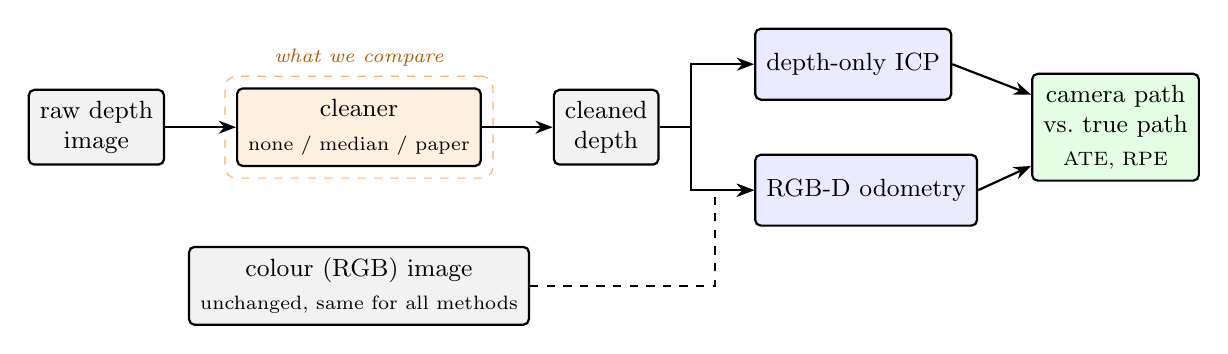
\begin{tikzpicture}[
  node distance=6mm and 9mm,
  box/.style={draw, rounded corners=2pt, align=center, font=\small, minimum height=9mm, inner sep=4pt},
  data/.style={box, fill=gray!10},
  proc/.style={box, fill=orange!12},
  trk/.style={box, fill=blue!8},
  eval/.style={box, fill=green!10},
  >={Stealth[length=2.2mm]}, thick]
  \node[data] (depth) {raw depth\\image};
  \node[proc, right=of depth] (clean) {cleaner\\[1pt]\scriptsize none / median / paper};
  \node[data, right=of clean] (cd) {cleaned\\depth};
  \node[trk, right=12mm of cd, yshift=8mm] (icp) {depth-only ICP};
  \node[trk, right=12mm of cd, yshift=-8mm] (rgbd) {RGB-D odometry};
  \node[data, below=10mm of clean] (rgb) {colour (RGB) image\\[1pt]\scriptsize unchanged, same for all methods};
  \node[eval, right=10mm of icp, yshift=-8mm] (path) {camera path\\vs.\ true path\\[1pt]\scriptsize ATE, RPE};
  \draw[->] (depth) -- (clean);
  \draw[->] (clean) -- (cd);
  \draw[->] (cd.east) -- ++(4mm,0) |- (icp.west);
  \draw[->] (cd.east) -- ++(4mm,0) |- (rgbd.west);
  \draw[->, dashed] (rgb.east) -| ([xshift=-5mm]rgbd.west) -- (rgbd.west);
  \draw[->] (icp.east) -- (path);
  \draw[->] (rgbd.east) -- (path);
  \begin{scope}[on background layer]
    \node[draw=orange!60, dashed, rounded corners, fit=(clean), inner sep=4pt,
          label={[font=\scriptsize\itshape, text=orange!70!black]above:what we compare}] {};
  \end{scope}
\end{tikzpicture}
\caption{Experiment pipeline. Only the cleaner changes between runs. The colour image skips the cleaner and goes
straight to the RGB-D tracker, identical for every method.}
\label{fig:pipeline}
\end{figure}

\paragraph{Why test with an RGB-D tracker at all?}
Real systems use both kinds of tracker: depth-only systems (KinectFusion-style ICP) and colour-plus-depth
systems (most modern RGB-D SLAM). A depth cleaner is only useful if it helps the tracker it is plugged into.
Testing both turned out to matter, since the best cleaner is different for each (Section~\ref{sec:tracking}).
\begin{itemize}
  \item \textbf{Depth-only ICP}: Open3D point-to-plane ICP between consecutive point clouds, three levels
        (voxel 4/2/1\cm, max.\ match distance 10/5/2\cm, 30 iterations each), starting from the previous motion.
        It uses the depth only.
  \item \textbf{RGB-D odometry}: Open3D hybrid odometry, which combines a photometric (colour) term and a geometric
        (depth) term. It uses the depth to project \emph{every} pixel into the next frame, so wrong depth values
        affect it directly.
\end{itemize}
Both trackers align consecutive frames and chain the motions into a path.

\subsection{Data}

\begin{table}[h]
\centering\small
\begin{tabular}{@{}L{4.4cm}L{3.6cm}lL{4.5cm}@{}}
\toprule
dataset & type & frames & ground truth \\
\midrule
ICL-NUIM living room kt0 \cite{icl} & synthetic, simulated Kinect noise & 1--300 & true depth \emph{and} true camera path \\
TUM RGB-D fr3 long\_office\_household \cite{tum} & real Asus Xtion sensor & 0--299 & true camera path (motion capture), no true depth \\
\bottomrule
\end{tabular}
\caption{Datasets. Every 2nd frame is tracked (150 frames per sequence). TUM has no true depth, so depth accuracy is
measured on ICL only. The camera moves 6.5\mm per tracked step on ICL (0.97\,m in total) and 20.7\mm on TUM
(3.09\,m).}
\label{tab:data}
\end{table}

\subsection{Metrics}

\begin{table}[h]
\centering\small
\begin{tabular}{@{}lL{9.5cm}l@{}}
\toprule
metric & meaning & better \\
\midrule
MAE (mm) & mean $|d - d^*|$ over pixels with a value, $d$ cleaned and $d^*$ true depth & lower \\
RMSE (mm) & $\sqrt{\text{mean}\,(d - d^*)^2}$; large errors count more. RMSE $\gg$ MAE means spikes remain & lower \\
within 1\cm (\%) & share of pixels less than 10\mm from the true depth & higher \\
ATE (cm) & absolute trajectory error: RMS distance between estimated and true camera positions after the best rigid
alignment of the whole path. Measures overall drift & lower \\
RPE (mm) & relative pose error: RMS error of each single step between tracked frames. Measures local accuracy and does
not accumulate & lower \\
\bottomrule
\end{tabular}
\caption{Metrics. Depth metrics are averaged over the 300 ICL frames; pixels a method leaves as holes are not scored.
Differences below about 0.05\cm ATE are within run-to-run noise.}
\label{tab:metrics}
\end{table}

% ---------------------------------------------------------------------------
\section{Results}

\subsection{Depth accuracy (ICL)}

\begin{table}[h]
\centering\small
\begin{tabular}{@{}lcccc@{}}
\toprule
method & MAE (mm) & RMSE (mm) & median error (mm) & within 1\cm (\%) \\
\midrule
no cleaning (input)            & 39.19 & 187.45 & 13.33 & 42.19 \\
\textcolor{ours}{\textbf{median 9$\times$9 (ours)}} & \best{18.77} & \best{55.41} & \best{12.32} & \best{44.66} \\
median 9$\times$9 + Telea fill & 19.34 & 57.67 & 12.36 & 44.47 \\
\textcolor{paper}{\textbf{paper (Fu et al.)}} & 37.69 & 186.00 & 13.42 & 33.69 \\
\bottomrule
\end{tabular}
\caption{ICL depth error against the true depth, mean over 300 frames. Bold: best per column.}
\label{tab:depth}
\end{table}

\noindent
\textbf{The median halves the depth error; the paper's pipeline barely changes it.} The input's RMSE (187\mm) is almost
five times its MAE (39\mm), so the ICL noise is dominated by spikes. The median removes them (RMSE drops to 55\mm),
and it lowers the error on every one of the 300 frames. The paper's bilateral filter weights each neighbour by how
similar its depth is to the centre pixel, so a spike is only averaged with itself and survives (RMSE 186\mm).
The paper's output is smoother, but its error grows with distance (its smoothing widens as $\Theta(z)$ grows), so fewer
pixels end up within 1\cm (33.7\,\% vs.\ 44.7\,\%). Figure~\ref{fig:depth} shows one frame.

\begin{figure}[h]
\centering
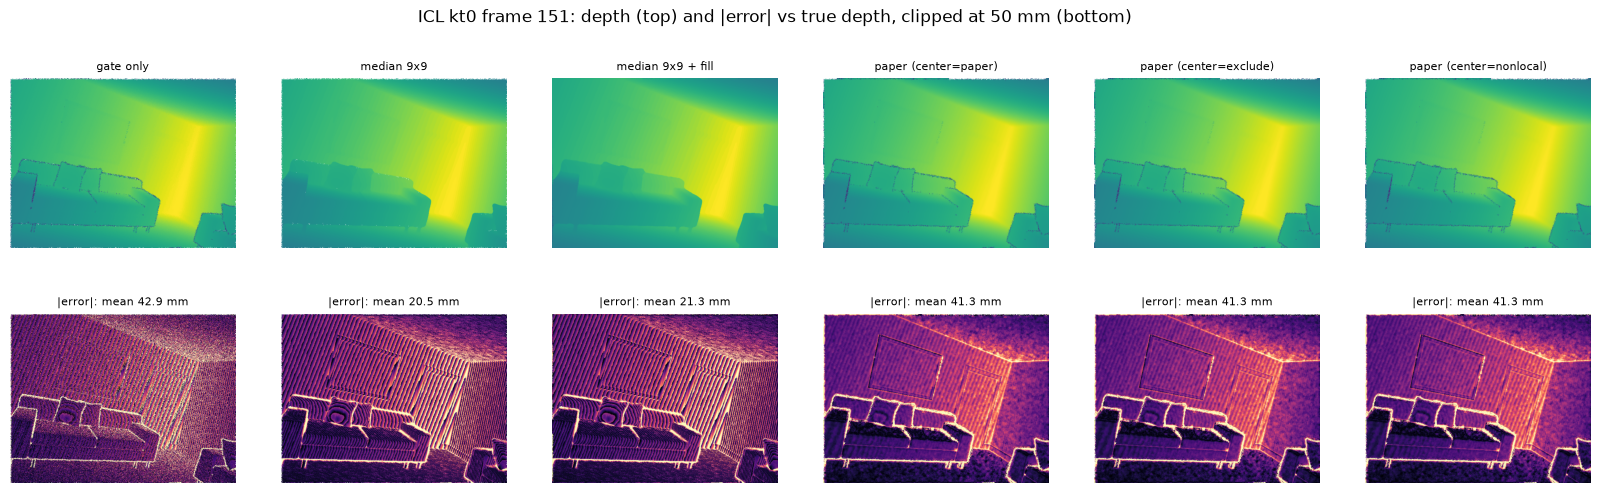
\includegraphics[width=\linewidth]{../src/results/icl_depth_example.png}
\caption{ICL frame 151. Top: depth after each method. Bottom: absolute error against the true depth (brighter = worse,
clipped at 50\mm). The median removes the speckled spikes but keeps the sensor's striped error pattern; the paper's
output is smooth but keeps the spikes and the edge errors.}
\label{fig:depth}
\end{figure}

\subsection{Camera tracking}
\label{sec:tracking}

\begin{table}[h]
\centering\small
\setlength{\tabcolsep}{5pt}
\begin{tabular}{@{}lcccccccc@{}}
\toprule
 & \multicolumn{4}{c}{ICL-NUIM kt0} & \multicolumn{4}{c}{TUM fr3 long\_office\_household} \\
\cmidrule(lr){2-5}\cmidrule(l){6-9}
 & \multicolumn{2}{c}{depth-only ICP} & \multicolumn{2}{c}{RGB-D odometry} & \multicolumn{2}{c}{depth-only ICP} & \multicolumn{2}{c}{RGB-D odometry} \\
\cmidrule(lr){2-3}\cmidrule(lr){4-5}\cmidrule(lr){6-7}\cmidrule(l){8-9}
method & ATE & RPE & ATE & RPE & ATE & RPE & ATE & RPE \\
\midrule
\textit{true depth (best possible)} & \textit{0.19} & \textit{0.07} & \textit{0.81} & \textit{2.18} & -- & -- & -- & -- \\
no cleaning (input)            & 17.07 & 14.43 & 23.59 & 24.20 & 13.97 & 11.69 & 2.14 & \best{5.61} \\
\textcolor{ours}{\textbf{median 9$\times$9 (ours)}} & 14.94 & 11.78 & \best{0.98} & \best{1.59} & 13.32 & 10.86 & \best{2.08} & 5.69 \\
median 9$\times$9 + Telea fill & 15.18 & 12.01 & 1.44 & 1.91 & 20.20 & 12.46 & 3.13 & 5.69 \\
\textcolor{paper}{\textbf{paper (Fu et al.)}} & \best{0.95} & \best{2.02} & 26.07 & 21.76 & \best{3.33} & \best{4.37} & 2.10 & 5.80 \\
\bottomrule
\end{tabular}
\caption{Camera path error over 150 tracked frames: ATE in cm, RPE in mm. Bold: best per column, not counting the
true-depth row, which tracks the noise-free ICL depth and shows the best each tracker can do.}
\label{tab:tracking}
\end{table}

\begin{keybox}[title=The result flips with the tracker]
\textbf{Depth-only ICP:} the paper's pipeline wins clearly (ATE 0.95 vs.\ 14.94\cm on ICL, 3.33 vs.\ 13.32\cm on TUM).\\
\textbf{RGB-D odometry:} the median wins on ICL (0.98\cm, close to the 0.81\cm limit) and ties on TUM;
the paper's pipeline does worse than no cleaning on ICL (26.1\cm).
\end{keybox}

\paragraph{Why the paper wins with depth-only ICP.}
Point-to-plane ICP discards point pairs that are far apart, so the spikes the paper leaves behind cost little. ICP also
relies on surface normals, which need smooth surfaces. The paper's bilateral smoothing gives clean surfaces and
good normals. The median leaves the sensor's striped error pattern (Figure~\ref{fig:depth}), which biases every
alignment step slightly in the same direction. No single step fails; the small biases add up to drift. With ICP, the median
improves only a little on the raw input (14.94 vs.\ 17.07\cm on ICL).

\paragraph{Why the median wins with RGB-D odometry.}
RGB-D odometry uses each pixel's depth to project it into the next frame and then compares colours. A spike sends its
pixel to the wrong place, and since nothing discards it, it pulls the estimate. The median removes the spikes, so
the tracker gets close to its noise-free result (0.98 vs.\ 0.81\cm). The paper's output keeps them, and the tracker
does slightly worse than with no cleaning at all. Figure~\ref{fig:paths} shows the effect.

\paragraph{TUM (real sensor).}
With RGB-D odometry all three main methods land within 0.06\cm of each other (2.08--2.14\cm), so cleaning makes
little difference there. This is consistent with the real sensor's noise being less spike-heavy than ICL's
simulated noise, but we did not test that directly. The depth-only ICP result (paper 4$\times$ better) holds on
real data too.

\begin{figure}[p]
\centering
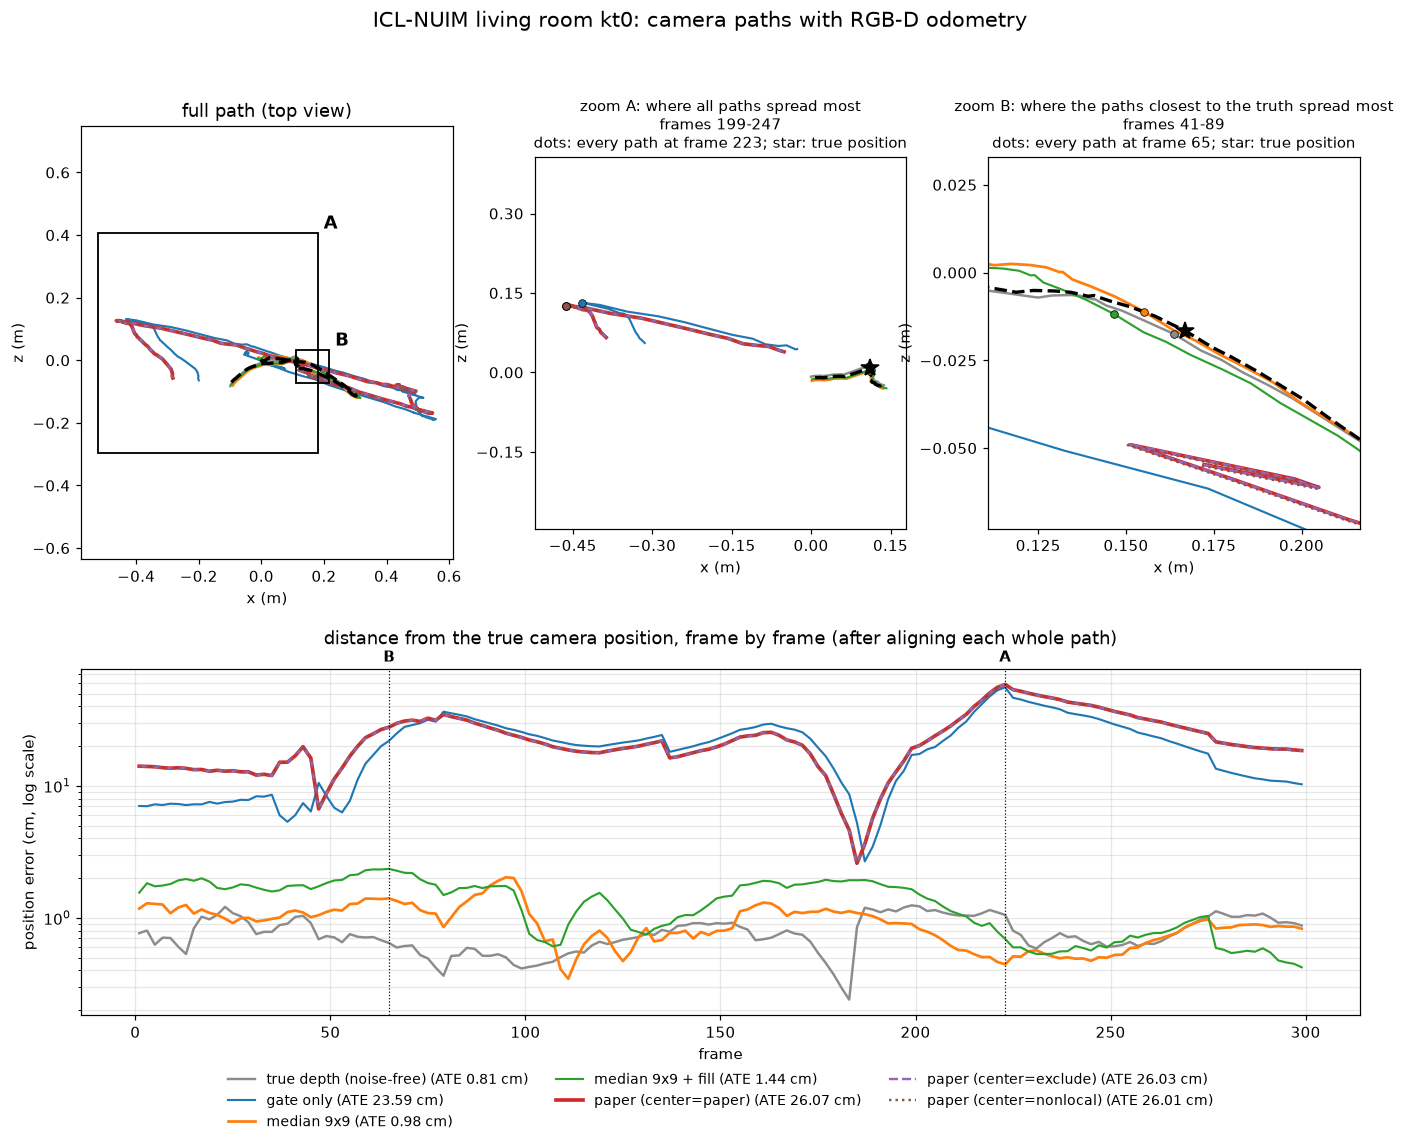
\includegraphics[width=0.92\linewidth]{../src/results/icl_paths_rgbd_zoom.png}
\caption{ICL, RGB-D odometry. Top: estimated camera paths seen from above, with two zoomed regions. Bottom: position
error per frame (log scale). The median (orange) stays near the true path; the paper's output (red) drifts as
much as the uncleaned input (blue). The three paper readings coincide.}
\label{fig:paths}
\end{figure}

\begin{figure}[p]
\centering
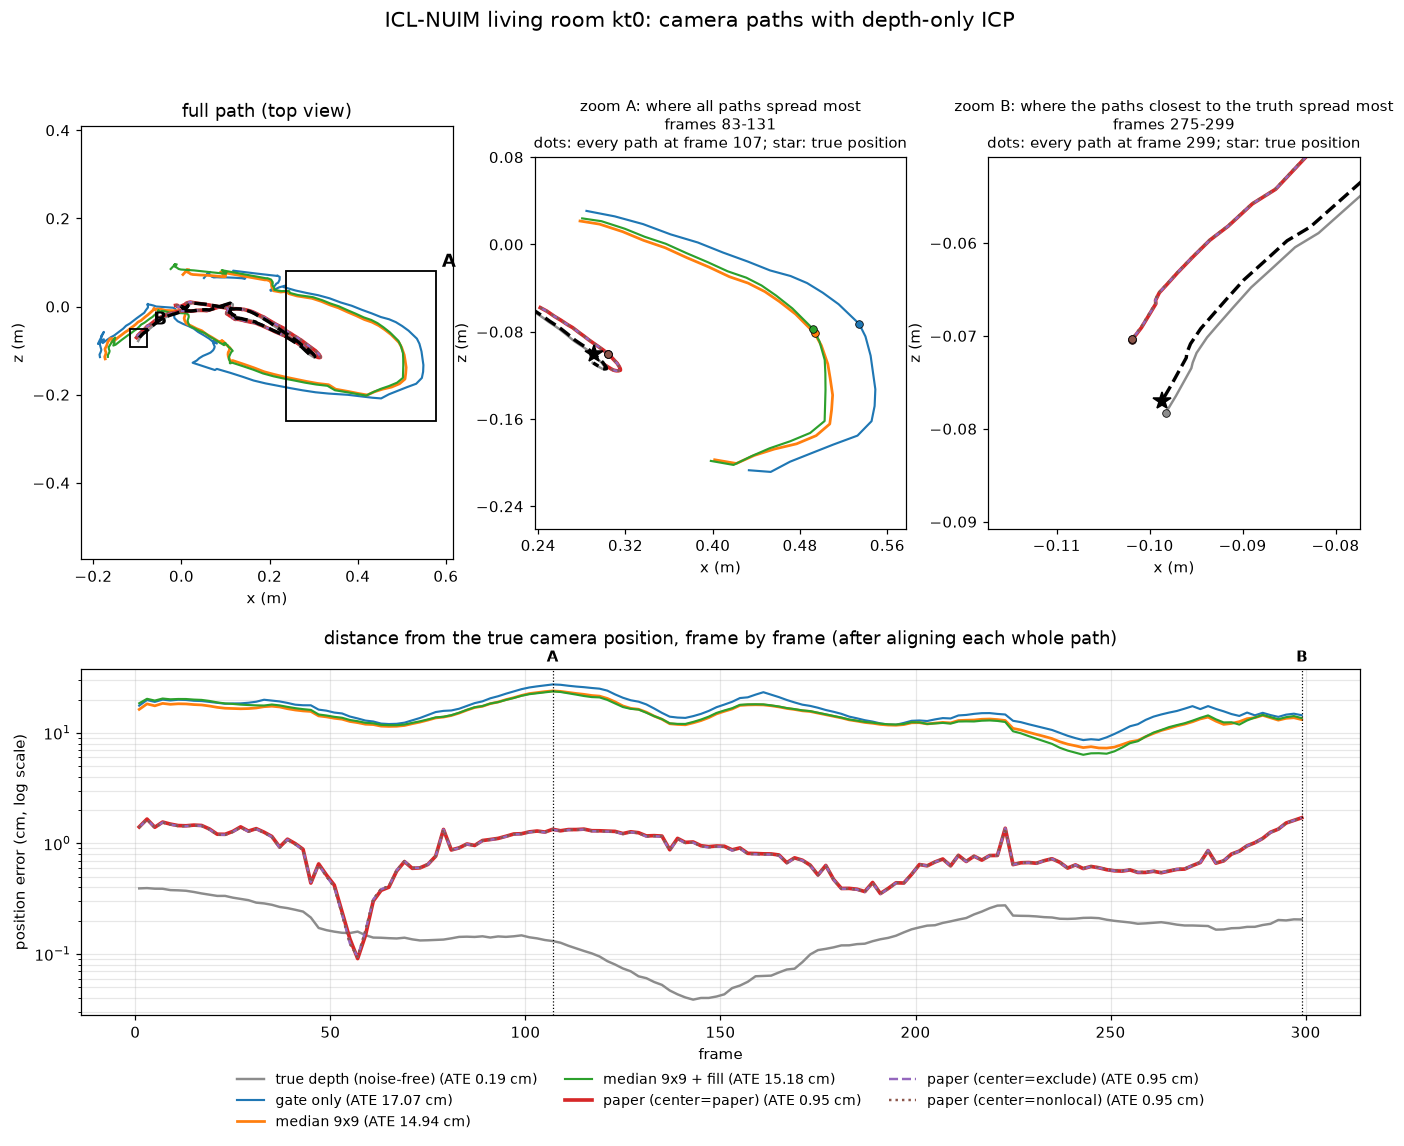
\includegraphics[width=0.92\linewidth]{../src/results/icl_paths_depth_zoom.png}
\caption{ICL, depth-only ICP, panels as in Figure~\ref{fig:paths}. Here the order is reversed: the paper's output
(red) tracks closely, while the median and the input drift.}
\label{fig:paths_icp}
\end{figure}

\subsection{Should the remaining holes be filled?}

After the median, about 1\,\% of ICL pixels and 16\,\% of TUM pixels are still holes. We tested eight ways to fill
them (\texttt{experiments/hole\_filling/}). Fill error is measured against the true depth at ICL's real holes.

\begin{table}[h]
\centering\small
\setlength{\tabcolsep}{4.5pt}
\begin{tabular}{@{}lcccccc@{}}
\toprule
 & fill error & \multicolumn{2}{c}{ICL ATE (cm)} & \multicolumn{2}{c}{TUM ATE (cm)} & time per \\
\cmidrule(lr){3-4}\cmidrule(lr){5-6}
fill method (after the median) & ICL (mm) & ICP & RGB-D & ICP & RGB-D & frame (TUM) \\
\midrule
\textbf{none (keep holes)}            & --  & \best{14.94} & \best{0.98} & 13.33 & \best{2.08} & 0\,ms \\
Telea inpainting (OpenCV)             & 87.0 & 15.18 & 1.44 & 20.21 & 3.13 & 210\,ms \\
Navier--Stokes inpainting (OpenCV)    & 22.5 & 15.36 & 1.46 & \best{12.03} & 3.89 & 224\,ms \\
nearest measured pixel                & 22.3 & 15.05 & 1.43 & 17.54 & 4.16 & 50\,ms \\
region growing, small holes only      & 15.5 & \best{14.94} & 1.01 & 13.32 & 2.23 & 52\,ms \\
region growing, median of neighbours  & 22.5 & 15.15 & 1.43 & 15.14 & 4.08 & 386\,ms \\
background (far side of the hole)     & 83.1 & 15.24 & 1.80 & 13.51 & 3.14 & 40\,ms \\
temporal (paper's prediction, $t\pm2$) & \best{12.2} & 15.11 & 1.24 & 13.37 & 2.51 & 7.9\,s \\
\bottomrule
\end{tabular}
\caption{Hole-filling methods. The ``small holes only'' fill fills just 4\,\% of ICL hole pixels and the temporal
fill 88.5\,\%, which flatters their fill error. Full numbers, including a masked test on both datasets, are in
\texttt{experiments/hole\_filling/results/fills.txt}.}
\label{tab:fills}
\end{table}

\noindent
\textbf{No fill improves RGB-D odometry, on either dataset.} A filled pixel is a guess, and the trackers do better
ignoring a missing pixel than using a wrong one. The fills that change the least (small holes only, temporal) do
the least harm. Telea inpainting, the obvious first choice, is among the least accurate (87\mm), because it blends the
near and far sides of a depth edge. The one improvement, Navier--Stokes with ICP on TUM (12.03 vs.\ 13.33\cm), is
reversed on ICL (15.36 vs.\ 14.94\cm), so we do not count it.

\begin{figure}[h]
\centering
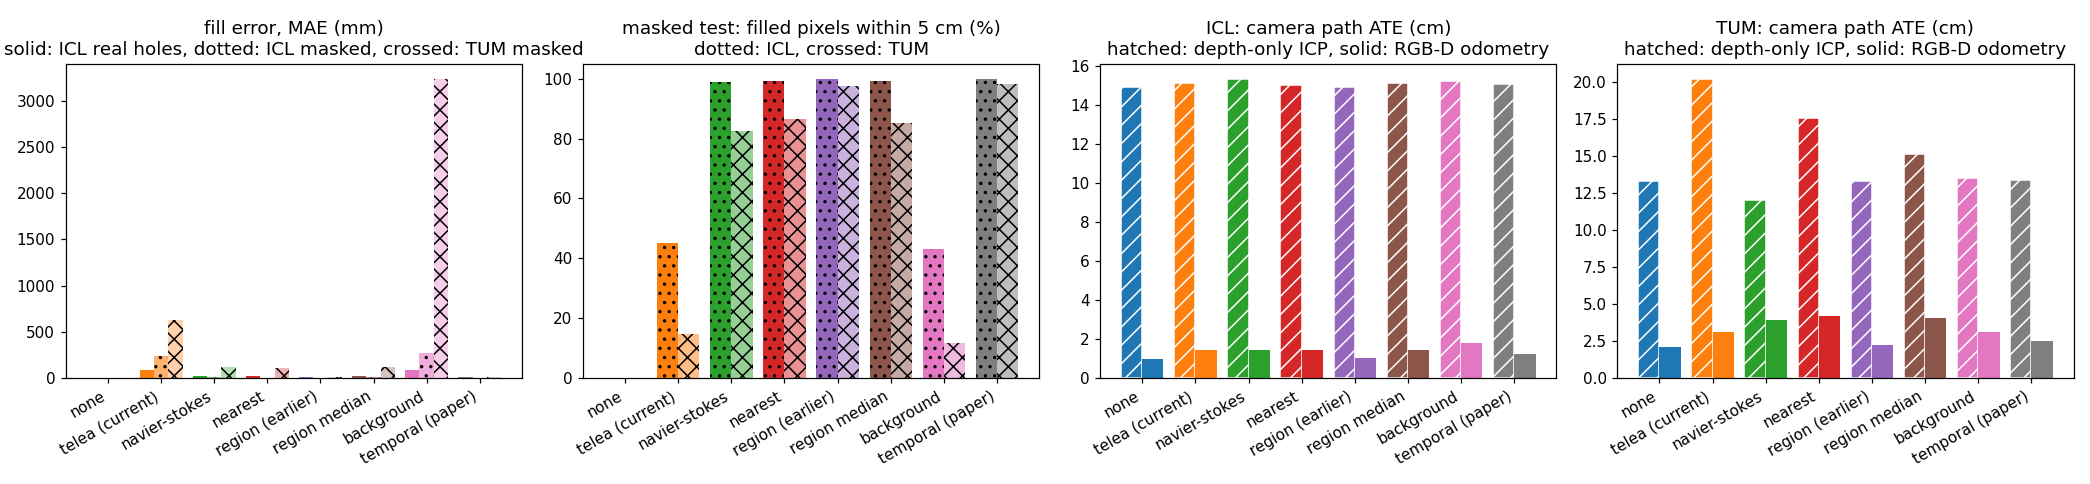
\includegraphics[width=\linewidth]{../experiments/hole_filling/results/fills.png}
\caption{Fill error (left two panels) and camera path ATE (right two panels) for each fill method.}
\label{fig:fills}
\end{figure}

% ---------------------------------------------------------------------------
\section{Discussion}

\paragraph{Depth accuracy does not predict tracking accuracy.}
The median is far more accurate per pixel, yet it loses badly with depth-only ICP. What ICP needs is smooth surfaces
with consistent normals; what RGB-D odometry needs is the absence of wild outliers. Judging a depth cleaner by
MAE alone, or by how the output looks, would give the wrong recommendation for one of the two trackers.

\paragraph{Cost.}
For 450 frames the median takes under a minute; the paper's pipeline takes about 26 minutes, mostly in block matching.
The median can run in real time; the paper's pipeline as implemented here cannot.

\paragraph{Limitations.}
\begin{itemize}
  \item One sequence per dataset, 150 tracked frames each. The large differences (4--16$\times$ in ATE) are robust;
        differences of a few millimetres are not.
  \item ICL's noise is simulated. The real sensor (TUM) shows much smaller differences between cleaners with RGB-D
        odometry.
  \item TUM has no true depth, so depth accuracy is measured on synthetic data only.
  \item The trackers are frame-to-frame with no loop closure or keyframes; a full SLAM system would correct part of
        the drift.
  \item Our re-implementation of Fu et al.\ may differ from the authors' code in details the paper does not give;
        we covered the main ambiguity (Eq.\ 7) with three readings.
\end{itemize}

% ---------------------------------------------------------------------------
\section{Conclusion}

\begin{table}[h]
\centering\small
\begin{tabular}{@{}L{3.6cm}L{4.9cm}L{6.6cm}@{}}
\toprule
if your system uses \dots & use & why \\
\midrule
RGB-D odometry (colour + depth) & \textcolor{ours}{\textbf{9$\times$9 median, no hole filling}} & error halved, best or equal-best tracking, $<$1 min \\
depth-only ICP & \textcolor{paper}{\textbf{Fu et al.\ pipeline}} & 4--16$\times$ less drift, but about 26 min \\
filled depth for display & median + Navier--Stokes or nearest & about 4$\times$ more accurate than Telea \\
\bottomrule
\end{tabular}
\end{table}

\noindent
A simple per-frame median filter is the better default for colour-plus-depth tracking: it is more accurate, much
faster, and does not need future frames. The paper's spatial-temporal pipeline is worth its cost only when the
tracker uses depth alone. Filling holes does not help tracking; if filled depth is needed, avoid Telea inpainting.

% ---------------------------------------------------------------------------
\section*{Reproducing the results}
\small
\begin{verbatim}
pip install -r requirements.txt                            # Python 3.12
python src/icl_compare.py --start 1 --frames 300 --step 2  # ICL
python src/tum_compare.py --start 0 --frames 300 --step 2  # TUM (Kaggle)
python experiments/hole_filling/compare_fills.py --frames 300 --step 2
cd report; pdflatex report.tex; pdflatex report.tex        # this report
\end{verbatim}
\normalsize
Raw numbers are in:
\begin{itemize}
  \item \texttt{src/results/icl\_compare.txt} and \texttt{src/results/tum\_compare.txt}
  \item \texttt{experiments/hole\_filling/results/fills.txt}
\end{itemize}

% ---------------------------------------------------------------------------
\begin{thebibliography}{9}
\bibitem{fu2012} J.~Fu, S.~Wang, Y.~Lu, S.~Li, W.~Zeng, ``Kinect-like depth denoising,'' in \emph{Proc.\ IEEE ISCAS}, 2012.
\bibitem{icl} A.~Handa, T.~Whelan, J.~McDonald, A.~J.~Davison, ``A benchmark for RGB-D visual odometry, 3D reconstruction and SLAM,'' in \emph{Proc.\ IEEE ICRA}, 2014.
\bibitem{tum} J.~Sturm, N.~Engelhard, F.~Endres, W.~Burgard, D.~Cremers, ``A benchmark for the evaluation of RGB-D SLAM systems,'' in \emph{Proc.\ IEEE/RSJ IROS}, 2012.
\end{thebibliography}

% ---------------------------------------------------------------------------
\appendix
\section{The three readings of Eq.~7}
\label{app:readings}

\begin{table}[h]
\centering\small
\setlength{\tabcolsep}{5pt}
\begin{tabular}{@{}lccccccccc@{}}
\toprule
 & ICL MAE & \multicolumn{2}{c}{ICL ICP} & \multicolumn{2}{c}{ICL RGB-D} & \multicolumn{2}{c}{TUM ICP} & \multicolumn{2}{c}{TUM RGB-D} \\
\cmidrule(lr){3-4}\cmidrule(lr){5-6}\cmidrule(lr){7-8}\cmidrule(l){9-10}
reading & (mm) & ATE & RPE & ATE & RPE & ATE & RPE & ATE & RPE \\
\midrule
\texttt{paper}    & 37.69 & 0.95 & 2.02 & 26.07 & 21.76 & 3.33 & 4.37 & 2.10 & 5.80 \\
\texttt{exclude}  & 37.69 & 0.95 & 2.02 & 26.03 & 21.76 & 3.31 & 4.37 & 2.10 & 5.79 \\
\texttt{nonlocal} & 37.69 & 0.95 & 2.02 & 26.01 & 21.75 & 3.31 & 4.37 & 2.12 & 5.80 \\
\bottomrule
\end{tabular}
\caption{The three readings of the hole-prediction equation give the same results to within 0.06\cm ATE.}
\end{table}

\clearpage
\section{TUM camera paths}

\begin{figure}[h]
\centering
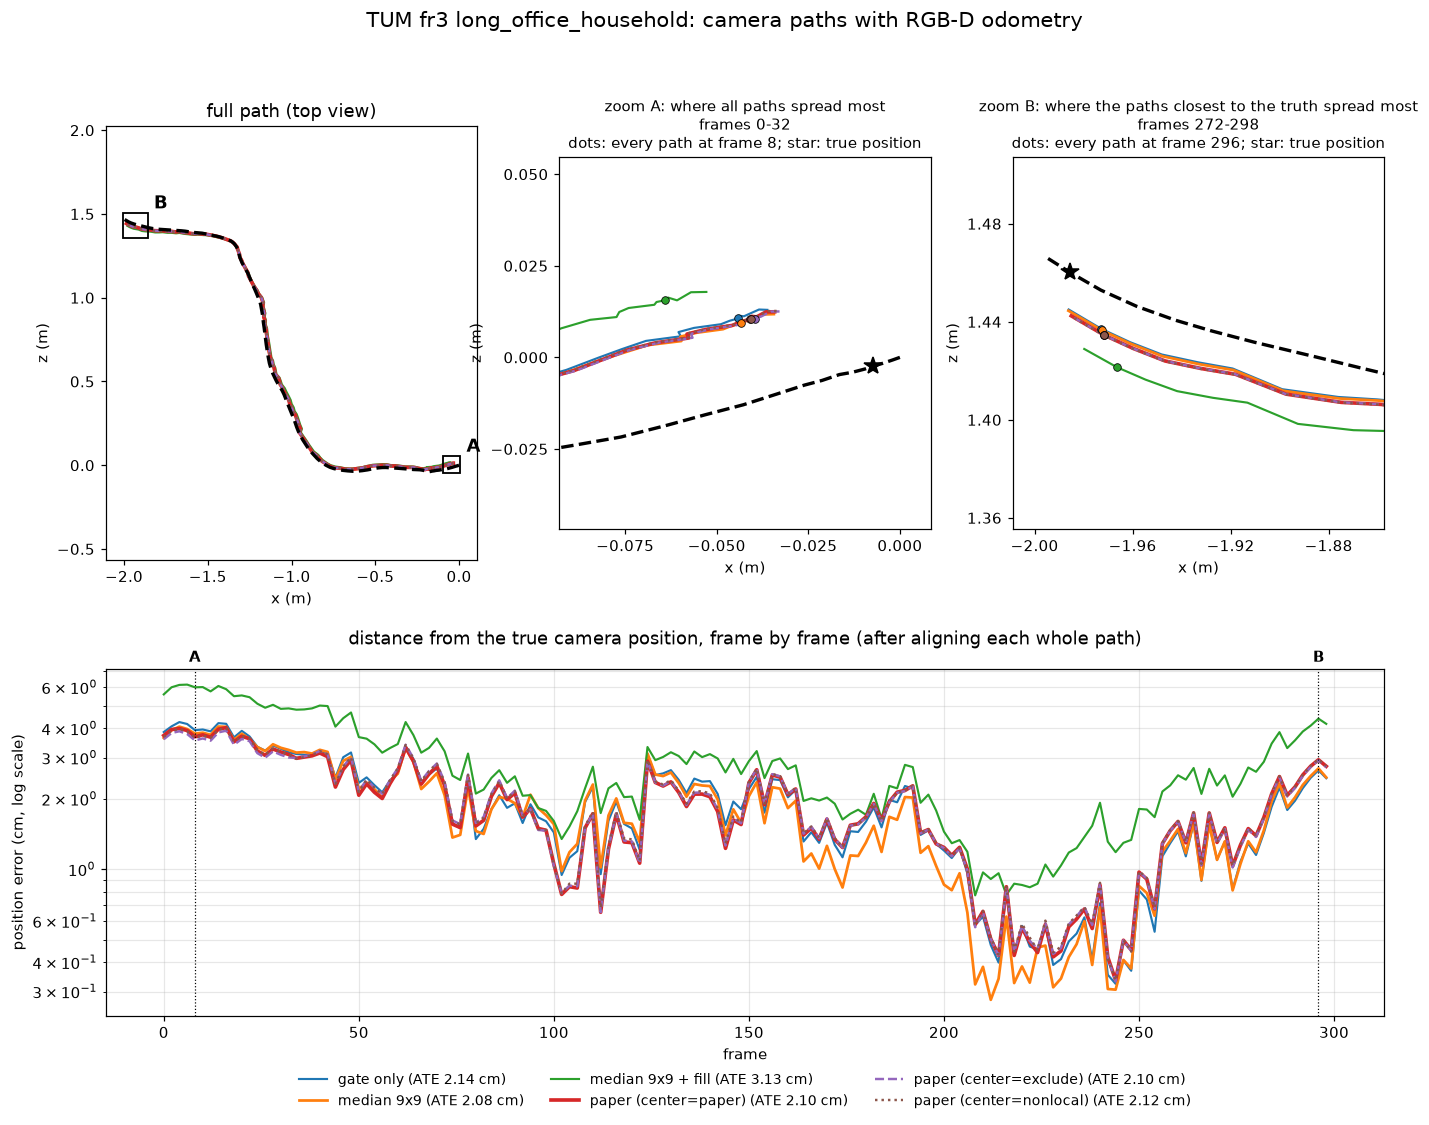
\includegraphics[width=0.8\linewidth]{../src/results/tum_paths_rgbd_zoom.png}
\caption{TUM, RGB-D odometry: input, median and paper stay close together (ATE 2.08--2.14\cm); the median with Telea
fill (green) drifts more (3.13\cm).}
\end{figure}

\begin{figure}[h]
\centering
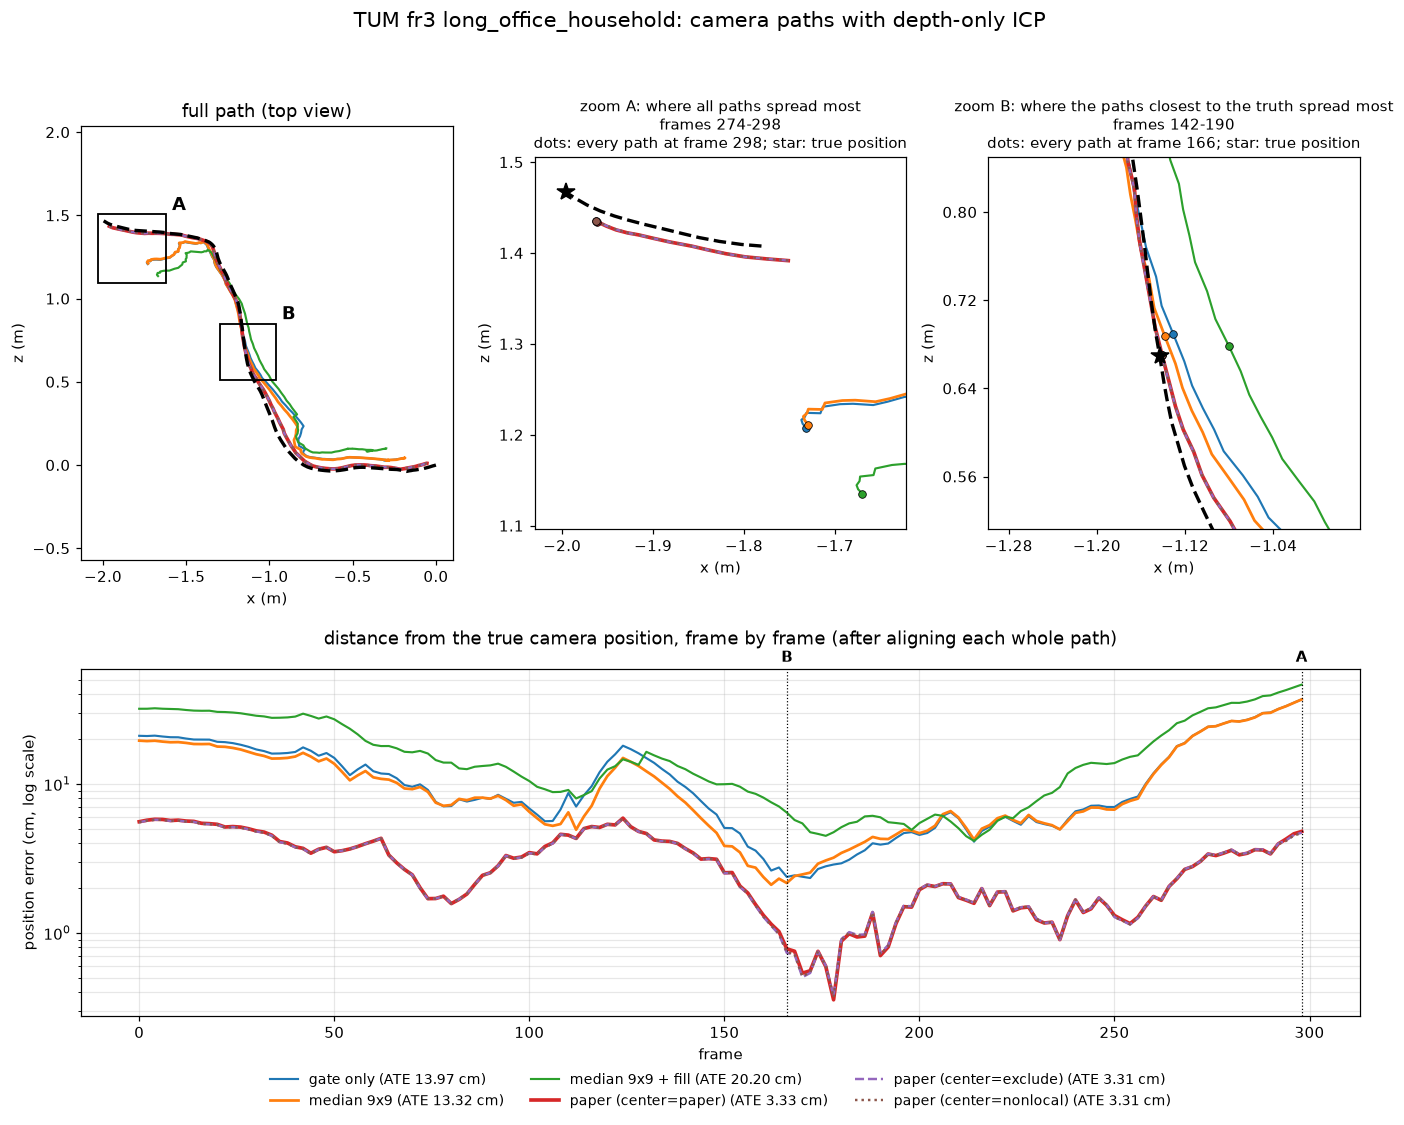
\includegraphics[width=0.8\linewidth]{../src/results/tum_paths_depth_zoom.png}
\caption{TUM, depth-only ICP: the paper's output (red) drifts much less than the median and the input.}
\end{figure}

\end{document}
